\documentclass[oneside,12pt]{article}          % ----- article

\input{../../../Latex/inputs/loading_packages.tex}			% ----- Packages utiles
\input{../../../Latex/inputs/preambule_exos.tex}         	% ----- Préambule feuilles de TD
\input{../../../Latex/inputs/mymacros.tex}                 % ----- Macros mathématiques
\input{../../../Latex/inputs/mise_en_page.tex} 		   	% ----- Macros de mise en page
\input{../../../Latex/inputs/macros_tikz.tex} 		   	% ----- Macros utiles TikZ

\fancyhead[R]{T\up{ale} Technologique}            % En-tête droit
\fancyhead[C]{Fonction inverse}


%%%%%%%%%%%%%%%%%%%%%%%%%%%%%%%%%%%%%%%%%%%%%%%%%%%%%%%%%%%%%%%%%%%%%%%%%%%%%%%%%%%%%%%%%%%%%%%%%%%%%%%%%%%%%
%%%%%%%%%%%%%%%%%%%%%%%%%%%%%%%%%%%%%%%%%%%%%%%%%%%%%%%%%%%%%%%%%%%%%%%%%%%%%%%%%%%%%%%%%%%%%%%%%%%%%%%%%%%%%
%%%%%%%%%%%%%%%%%%%%%%%%%%%%%%%%%%%%%%%%%%%%%%%%%%%%%%%%%%%%%%%%%%%%%%%%%%%%%%%%%%%%%%%%%%%%%%%%%%%%%%%%%%%%%


\begin{document}

\section{Tableaux de signes}

\subsection{Produit direct}
Dresser le tableau de signes des fonctions suivantes :

\begin{tabular}{p{0.3\linewidth} p{0.3\linewidth} p{0.3\linewidth}}
$f:x\mapsto (3x-6)(2+x)$ & $g:x\mapsto (4-2x)(x+3)$ & $h:x\mapsto (2+2x)(3-x)$
\end{tabular}



\subsection{Quotient direct}
Dresser le tableau de signes des fonctions suivantes :

\begin{tabular}{p{0.3\linewidth} p{0.3\linewidth} p{0.3\linewidth}}
$f:x\mapsto \dfrac{x+2}{5-x}$ & $g:x\mapsto \dfrac{10-5x}{4+2x}$ & $h:x\mapsto \dfrac{2x+8}{2x+5}$
\end{tabular}



\subsection{Association}
Associer chacune des fonctions suivantes à son tableau de signes :

\begin{center}
	\renewcommand{\arraystretch}{1.5}
	\begin{tabular}{p{0.3\linewidth} p{0.3\linewidth} p{0.3\linewidth}}
	$f_1:x\mapsto (x-3)(x-2)$ & $f_2:x\mapsto (x+3)(2-x)$ & $f_3:x\mapsto (3-x)(2+x)$ \\
	$f_4:x\mapsto (3+x)(2+x)$ & $f_5:x\mapsto (x+3)(x-2)$ & $f_6:x\mapsto (3-x)(x-2)$
	\end{tabular}
	
	\begin{tikzpicture}
		\tkzTabInit[espcl=2 , lgt = 1.5 , color , colorL=gray!25 , colorV=gray!25]{$x$ /0.75 ,  /1}%
		{$-\infty$ , $2$ , $3$ , $+\infty$}%
		\tkzTabLine{ , - , z , + , z , -}
	\end{tikzpicture} \hspace{1cm}
	\begin{tikzpicture}
		\tkzTabInit[espcl=2 , lgt = 1.5 , color , colorL=gray!25 , colorV=gray!25]{$x$ /0.75 ,  /1}%
		{$-\infty$ , $2$ , $3$ , $+\infty$}%
		\tkzTabLine{ , + , z , - , z , +}
	\end{tikzpicture}
	
	\begin{tikzpicture}
		\tkzTabInit[espcl=2 , lgt = 1.5 , color , colorL=gray!25 , colorV=gray!25]{$x$ /0.75 ,  /1}%
		{$-\infty$ , $-3$ , $-2$ , $+\infty$}%
		\tkzTabLine{ , + , z , - , z , +}
	\end{tikzpicture} \hspace{1cm}
	\begin{tikzpicture}
		\tkzTabInit[espcl=2 , lgt = 1.5 , color , colorL=gray!25 , colorV=gray!25]{$x$ /0.75 ,  /1}%
		{$-\infty$ , $-3$ , $2$ , $+\infty$}%
		\tkzTabLine{ , + , z , - , z , +}
	\end{tikzpicture}
	
	\begin{tikzpicture}
		\tkzTabInit[espcl=2 , lgt = 1.5 , color , colorL=gray!25 , colorV=gray!25]{$x$ /0.75 ,  /1}%
		{$-\infty$ , $-3$ , $2$ , $+\infty$}%
		\tkzTabLine{ , - , z , + , z , -}
	\end{tikzpicture} \hspace{1cm}
	\begin{tikzpicture}
		\tkzTabInit[espcl=2 , lgt = 1.5 , color , colorL=gray!25 , colorV=gray!25]{$x$ /0.75 ,  /1}%
		{$-\infty$ , $-2$ , $3$ , $+\infty$}%
		\tkzTabLine{ , - , z , + , z , -}
	\end{tikzpicture}
\end{center}



\section{Tableaux de variation}

\subsection{Incohérences}
On a dressé ci-après plusieurs tableaux.

Expliquer pourquoi aucun d'entre eux ne peut être un tableau de variations cohérent.

\begin{minipage}{0.5\linewidth}
	\begin{tikzpicture}
		\tkzTabInit[color , colorL=gray!25 , colorV=gray!25 , espcl=2]
			{$x$ / 1 , $f(x)$ / 2} {$-7$ , $8$ , $1$ , $15$}
		\tkzTabVar{-/ $-2$ , +/ ${1,4}$ , -/ $-1$ , +/ $4$}
	\end{tikzpicture}\vspace{3mm}
	\begin{tikzpicture}
		\tkzTabInit[color , colorL=gray!25 , colorV=gray!25 , espcl=3]
			{$x$ / 1 , $h(x)$ / 2} {$-2$ , $3$ , ${8,1}$ }
		\tkzTabVar{-/ ${0,16}$ , +/ $4$ , -/ ${5,2}$ }
	\end{tikzpicture}
\end{minipage} \hspace{3mm}
\begin{minipage}{0.5\linewidth}
	\begin{tikzpicture}
		\tikzset{arrow style/.style = {\tkzTabDefaultWritingColor,Stealth-,> = \tkzTabDefaultArrowStyle,shorten > = \tkzTabDefaultSep,shorten < = \tkzTabDefaultSep}}
		\tkzTabInit[color , colorL=gray!25 , colorV=gray!25 , espcl=2]
			{$x$ / 1 , $g(x)$ / 2} {$-5$ , $1$ , $4$ , $11$}
		\tkzTabVar{+/ $-1$ , -/ $3$ , +/ $0$ , -/ $7$}
	\end{tikzpicture}\vspace{3mm}
	\begin{tikzpicture}
		\tkzTabInit[color , colorL=gray!25 , colorV=gray!25 , espcl=2]
			{$x$ / 1 , $\phi(x)$ / 2} {{$0,1$} , $1$ , $11$ , $111$}
		\tkzTabVar{-/ $-2$ , +/ $\pi$ , -/ $\frac{22}{7}$ , +/ $7$}
	\end{tikzpicture}
\end{minipage}



\subsection{D'après le tracé}
On a tracé ci-après les courbes représentatives des fonctions $f$, $g$ et $h$.

\hspace{-3mm}
\begin{minipage}{0.33\linewidth}
    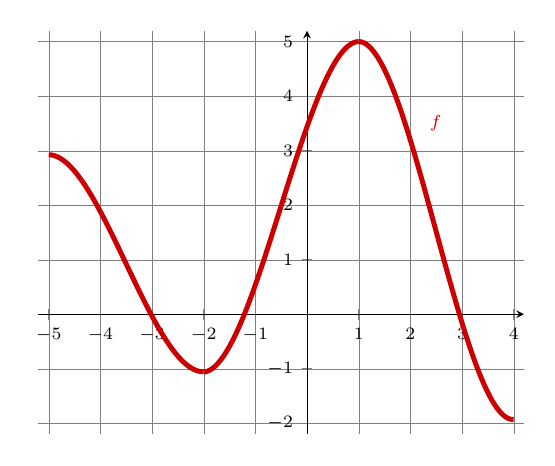
\begin{tikzpicture}[scale=0.9]
        \begin{axis}[xmin=-5 , xmax=4 , ymin=-2 , ymax=5,
        xtick distance = 1, ytick distance = 1,
        axis lines = middle, enlargelimits = { abs = 0.2},
    	grid=major , major grid style = {line width = 0.1pt ,draw = gray}, 
        ticklabel style = {font = \scriptsize }
        ]
        
        \addplot[color=red!80!black , samples = 100 , domain = -5:-2 , line width = 2pt]
        {0.2956*x^3+3.11*x^2+8.915*x+6.7};
        \addplot[color=red!80!black , samples = 100 , domain = -2:1 , line width = 2pt]
        {-0.44*x^3-0.67*x^2+2.67*x+3.44};
        \addplot[color=red!80!black , samples = 100 , domain = 1:4 , line width = 2pt]
        {0.52*x^3-3.89*x^2+6.22*x+2.15};
        
        \draw[color=red!80!black] (2.5,3.5) node {$\Ccal_f$};

    	\end{axis}
    \end{tikzpicture}
\end{minipage} \hspace{1mm}
\begin{minipage}{0.33\linewidth}
    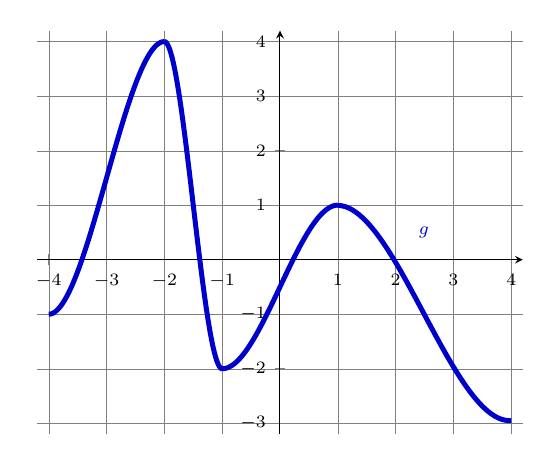
\begin{tikzpicture}[scale=0.9]
        \begin{axis}[xmin=-4 , xmax=4 , ymin=-3 , ymax=4,
        xtick distance = 1, ytick distance = 1,
        axis lines = middle, enlargelimits = { abs = 0.2},
    	grid=major , major grid style = {line width = 0.1pt ,draw = gray}, 
        ticklabel style = {font = \scriptsize }
        ]
        
        \addplot[color=blue!80!black , samples = 100 , domain = -4:-2 , line width = 2pt]
        {-1.25*x^3-11.25*x^2-30*x-21};
        \addplot[color=blue!80!black , samples = 100 , domain = -2:-1 , line width = 2pt]
        {12*x^3+54*x^2+72*x+28};
        \addplot[color=blue!80!black , samples = 100 , domain = -1:1 , line width = 2pt]
        {-0.75*x^3+2.25*x-0.5};
        \addplot[color=blue!80!black , samples = 100 , domain = 1:4 , line width = 2pt]
        {0.3*x^3-2.235*x^2+3.56*x-0.63};
        
        \draw[color=blue!80!black] (2.5,0.5) node {$\Ccal_g$};

    	\end{axis}
    \end{tikzpicture}
\end{minipage} \hspace{1mm}
\begin{minipage}{0.33\linewidth}
    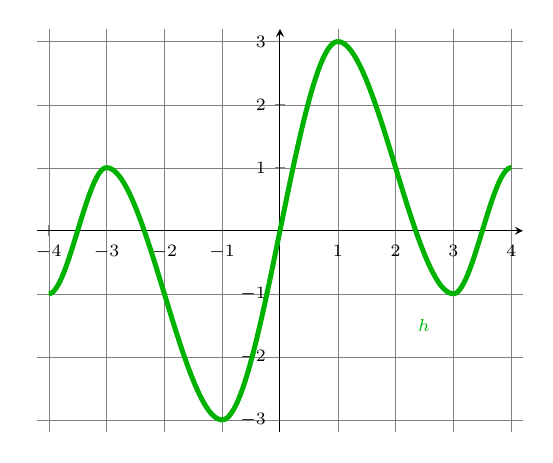
\begin{tikzpicture}[scale=0.9]
        \begin{axis}[xmin=-4 , xmax=4 , ymin=-3 , ymax=3,
        xtick distance = 1, ytick distance = 1,
        axis lines = middle, enlargelimits = { abs = 0.2},
    	grid=major , major grid style = {line width = 0.1pt ,draw = gray}, 
        ticklabel style = {font = \scriptsize }
        ]
        
        \addplot[color=green!70!black , samples = 100 , domain = -4:-3 , line width = 2pt]
        {-4*x^3-42*x^2-144*x-161};
        \addplot[color=green!70!black , samples = 100 , domain = -3:-1 , line width = 2pt]
        {x^3+6*x^2+9*x+1};
        \addplot[color=green!70!black , samples = 100 , domain = -1:1 , line width = 2pt]
        {-1.5*x^3+4.5*x};
        \addplot[color=green!70!black , samples = 100 , domain = 1:3 , line width = 2pt]
        {x^3-6*x^2+9*x-1};
        \addplot[color=green!70!black , samples = 100 , domain = 3:4 , line width = 2pt]
        {-4*x^3+42*x^2-144*x+161};
        
        \draw[color=green!70!black] (2.5,-1.5) node {$\Ccal_h$};

    	\end{axis}
    \end{tikzpicture}
\end{minipage}

Compléter les tableaux de variations suivants :

\begin{tikzpicture}
	\pgfsetstrokecolor{red!80!black}
	\tkzTabInit[color , colorV=red!80!black!15 , colorL=red!80!black!15 , espcl = 16/3]
		{ $x$ /0.75 , $f(x)$ /1.7}{$-5$ , {\dots} ,  {\dots} , $4$}
	\tkzTabVar
		{+/ \vphantom{I}\dots , -/ \dots , +/ \vphantom{I}\dots , -/ {\dots}}
\end{tikzpicture}

\begin{tikzpicture}
	\pgfsetstrokecolor{blue!80!black}
	\tkzTabInit[color , colorV=blue!80!black!15 , colorL=blue!80!black!15 , espcl = 4]
		{ $x$ /0.75 , $g(x)$ /1.7}{$-4$ ,  {\dots} , {\dots} , {\dots} ,$4$}
\end{tikzpicture}

\begin{tikzpicture}
	\pgfsetstrokecolor{green!70!black}
	\tkzTabInit[color , colorV=green!70!black!15 , colorL=green!80!black!15 , espcl = 16/5]
		{ $x$ /0.75 , $h(x)$ /1.7}{$-4$ , {\dots} , {\dots} , {\dots} , {\dots} , $4$}
\end{tikzpicture}



\section{Notion de dérivation}

\subsection{Lecture graphique}
\begin{minipage}{0.5\textwidth} \restoreskip
	On a tracé ci-contre $\Ccal_f$ la courbe représentative d'une fonction $f$ dérivable sur l'intervalle $[-4 ~;~ 3]$.
	
	La droite $T_A$ est la tangente à $\Ccal_f$ au point $A$.\\
	La droite $T_B$ est la tangente à $\Ccal_f$ au point $B$.
	
	À l'aide du graphique :
	\begin{enumerate}
		\item Déterminer la valeur de $f(-1)$ et $f'(-1)$
		\item Déterminer la valeur de $f(2)$ et $f'(2)$
	\end{enumerate}
\end{minipage}
\begin{minipage}{0.5\textwidth}
	\begin{tikzpicture}
		\begin{axis}[
			width = 11cm , height = 8cm ,
	        xmin = -4 , xmax = 3 , ymin = -3 , ymax = 4 , xtick distance = 1 , ytick distance = 1 ,
	        grid = major, major grid style = {line width = 0.2pt , draw = gray},
	        axis lines = middle, enlargelimits = { abs = 0.2 },
	        ticklabel style = {font = \scriptsize}
	        ]
	
			% Courbe représentative
			\addplot[color = newblue, line width = 2.5pt, domain = -4:3 , samples = 100]
	    		{x^2/2 + x/2 - 1};
	    	\draw[color = newblue] (-2.5,2) node {$\Ccal_f$} ;
	    		
			% Tangente en x = -1
			\addplot[color = newred, line width = 2pt, domain = -4:3]
			    {-0.5*x - 1.5};
			\draw[color = newred] (-1,-1) node {$\bullet$} node[below left] {$A$} (-3.5,-0.5) node{$T_A$} ;
			
			% Tangente en x = 2
			\addplot[color = newgreen, line width = 2pt, domain = -4:3]
			    {2.5*x - 3} ;
			\draw[color = newgreen] (2,2) node {$\bullet$} node[below right] {$B$} (1.5,-0.5) node{$T_B$} ;		
		\end{axis}
	\end{tikzpicture}  
\end{minipage}



\subsection{Dans un sens}
\begin{minipage}{0.5\textwidth}
	\begin{tikzpicture}
		\begin{axis}[
			width = 10cm , height = 6cm ,
	        xmin = -3 , xmax = 3 , ymin = -1 , ymax = 3 , xtick distance = 1 , ytick distance = 1 ,
	        grid = major, major grid style = {line width = 0.2pt , draw = gray},
	        axis lines = middle, enlargelimits = { abs = 0.2 },
	        ticklabel style = {font = \scriptsize}
	        ]
	
			% Courbe représentative
			\addplot[color = newred , line width = 2.5pt , domain = -3.5:3.5 , samples = 100]
	    		{0.25 * (x-2) * (x+1)};
	    	\draw[color = newred] (2.5,1.5) node {$\Ccal_{f'}$} ;
	    	
		\end{axis}
	\end{tikzpicture}  
\end{minipage} 
\begin{minipage}{0.5\textwidth} \restoreskip
	On considère une fonction $f$ définie et dérivable sur l'intervalle $[-3 ~;~ 3]$
	
	On a tracé dans le repère ci-contre la courbe de la fonction $f'$.

	\begin{enumerate}
		\item Dresser le tableau de signes de la fonction $f'$ sur l'intervalle $[-3 ~;~ 3]$
		\item En déduire le tableau de variations sur l'intervalle $[-3 ~;~ 3]$ de la fonction $f$
	\end{enumerate}
\end{minipage}



\subsection{Puis dans l'autre}
\begin{minipage}{0.5\textwidth} \restoreskip
	On considère une fonction $f$ définie et dérivable sur l'intervalle $[-3 ~;~ 3]$
	
	On a tracé dans le repère ci-contre la courbe de la fonction $g$.

	\begin{enumerate}
		\item Dresser le tableau de variations de la fonction $g$ sur l'intervalle $[-3 ~;~ 3]$
		\item En déduire le tableau de signe sur l'intervalle $[-3 ~;~ 3]$ de la fonction $g'$
	\end{enumerate}
\end{minipage} \hspace{5mm}
\begin{minipage}{0.5\textwidth}
	\begin{tikzpicture}
		\begin{axis}[
			width = 10cm , height = 7cm ,
	        xmin = -3 , xmax = 5 , ymin = -3 , ymax = 3 , xtick distance = 1 , ytick distance = 1 ,
	        grid = major, major grid style = {line width = 0.2pt , draw = gray},
	        axis lines = middle, enlargelimits = { abs = 0.2 },
	        ticklabel style = {font = \scriptsize}
	        ]
	
			% Courbe représentative
			\addplot[color = newblue , line width = 2.5pt , domain = -3.5:5.5 , samples = 100]
	    		{1/36 * (4*x^3 - 9*x^2 - 54*x) + 1};
	    	\draw[color = newblue] (4.5,1.5) node {$\Ccal_g$} ;
	    	
		\end{axis}
	\end{tikzpicture}  
\end{minipage} 



\subsection{Identification graphique}
\begin{minipage}{0.5\textwidth}
	\begin{tikzpicture}
		\begin{axis}[
			width = 10cm , height = 7cm ,
	        xmin = -4 , xmax = 5 , ymin = -2 , ymax = 5 , xtick distance = 1 , ytick distance = 1 ,
	        grid = major, major grid style = {line width = 0.2pt , draw = gray},
	        axis lines = middle, enlargelimits = { abs = 0.2 },
	        ticklabel style = {font = \scriptsize}
	        ]
	
			% Courbe représentative
			\addplot[color = newred , line width = 2.5pt , domain = -4.5:5.5 , samples = 100]
	    		{1/2 * (e^(x/2) *(-1 + x/2)^2 + e^2 *(x/2 - (x/2)^3/3))};
	    	\draw[color = newred] (2.5,3.5) node {$\Ccal_h$} ;
	    	
		\end{axis}
	\end{tikzpicture}
\end{minipage}
\begin{minipage}{0.5\textwidth} \restoreskip
	On a tracé dans le repère ci-contre $\Ccal_h$ la courbe représentative de la fonction $h$ définie et dérivable sur l'intervalle $[-2 ~;~ 2,5]$
	
	Parmi les trois courbes représentées ci-dessous, laquelle pourrait être celle de la fonction $h'$, la fonction dérivée de la fonction $h$ ? Justifier.
\end{minipage}

\begin{tikzpicture}
	\begin{axis}[
		width = 7.5cm , height = 6cm ,
        xmin = -4 , xmax = 5 , ymin = -2 , ymax = 5 , xtick distance = 1 , ytick distance = 1 ,
        grid = major, major grid style = {line width = 0.2pt , draw = gray},
        axis lines = middle, enlargelimits = { abs = 0.2 },
        ticklabel style = {font = \tiny}
        ]

		% Courbe représentative
		\addplot[color = newblue , line width = 2pt , domain = -4.5:5.5 , samples = 100]
    		{e^(x/2) * (5 - 2* x) + ((e^2)/8 + e^(x/2)/4) * x^2 - (e^2 * x^4)/192) - 7};
	\end{axis}
\end{tikzpicture}\hspace{5mm}
\begin{tikzpicture}
	\begin{axis}[
		width = 7.5cm , height = 6cm ,
        xmin = -4 , xmax = 5 , ymin = -2 , ymax = 5 , xtick distance = 1 , ytick distance = 1 ,
        grid = major, major grid style = {line width = 0.2pt , draw = gray},
        axis lines = middle, enlargelimits = { abs = 0.2 },
        ticklabel style = {font = \tiny}
        ]

		% Courbe représentative
		\addplot[color = newblue , line width = 2pt , domain = -4.5:5.5 , samples = 100]
    		{1/16 * (-e^2 + e^(x/2)) * (-4 + x^2)};
	\end{axis}
\end{tikzpicture}\hspace{5mm}
\begin{tikzpicture}
	\begin{axis}[
		width = 7.5cm , height = 6cm ,
        xmin = -4 , xmax = 5 , ymin = -2 , ymax = 5 , xtick distance = 1 , ytick distance = 1 ,
        grid = major, major grid style = {line width = 0.2pt , draw = gray},
        axis lines = middle, enlargelimits = { abs = 0.2 },
        ticklabel style = {font = \tiny}
        ]

		% Courbe représentative
		\addplot[color = newblue , line width = 2pt , domain = -4.5:5.5 , samples = 100]
    		{3 - 1/2 * (e^(x/2) *(-1 + x/2)^2 + e^2 *(x/2 - (x/2)^3/3))};
	\end{axis}
\end{tikzpicture}



\subsection{Étude d'une parabole}
Soit $f$ la fonction définie sur $\RR$ par $f(x)=-2x^2+8x+1$
\begin{enumerate}[itemsep = 0pt]
    \item 
    \begin{enumerate}
        \item Calculer $f'(x)$
        \item Étudier le signe de $f'(x)$
    \end{enumerate}
    \item 
    \begin{enumerate}
        \item Dresser le tableau de variations de $f$ sur $\mathbb{R}$.
        \item En déduire que $f$ admet un extremum sur $\mathbb{R}$.
        Préciser en quelle valeur de $x$ il est atteint.
    \end{enumerate}
\end{enumerate}



\subsection{Un degré de plus}
Soit $f$ la fonction définie sur l'intervalle $[-3 ~;~ 2]$ par $g(x)=2x^3+3x^2-12x+4$
\begin{enumerate}[itemsep = 0pt]
    \item
    \begin{enumerate}
        \item Calculer $g'(x)$
        \item Montrer que $g'(x)=6(x+2)(x-1)$ , \quad pour tout $x\in[-3 ~;~ 2]$ 
    \end{enumerate}
    \item
    \begin{enumerate}
        \item Étudier le signe de $g'(x)$ sur $[-3 ~;~ 2]$ et en déduire le tableau de variations de $g$.
        \item Déterminer les extremums de $g$ sur $[-3 ~;~ 2]$ et préciser en quelles valeurs de $x$ ils sont atteints.
    \end{enumerate}
\end{enumerate}



\subsection{Un exercice coton}

Une entreprise produit du tissu.

On modélise le coût total de production (en euros) par la fonction $f$ définie par
$$f(x) = 15x^3 - 120x^2 + 500x + 750$$
Où $x$ est la longueur de tissu fabriqué exprimée en kilomètre, $x$ étant compris entre 0 et 10.

Chaque kilomètre de tissu est vendu 680 euros.

On note $B(x)$ le bénéfice de l'entreprise, c'est-à-dire la différence entre la recette et le coût de production, pour la vente de $x$ kilomètres de tissu.
\begin{enumerate}[itemsep = 0pt]
    \item Quel est le bénéfice de l'entreprise pour la vente de 3 kilomètres de tissu ?
    \item Montrer que $B(x)=-15x^3+120x^2+180x-750$ \quad pour tout $x \in [0 ~;~ 10]$
    \item Donner une expression de $B'(x)$, où $B'$ désigne la fonction dérivée de la fonction $B$.
    \item Dresser le tableau de signes de $B'(x)$ sur $[0\,;\,10]$ puis le tableau de variations de la fonction $B$.
    \item Combien de kilomètres de tissu l'entreprise doit-elle produire afin d'obtenir un bénéfice maximal ?
\end{enumerate}



\section{Fonction inverse}

\subsection{Échauffement calculatoire}
Calculer les dérivées des fonctions suivantes, définies sur $]-\infty ~;~ 0[\bbigcup]0 ~;~ +\infty[$ :

\renewcommand{\arraystretch}{2}
\begin{tabular}{p{0.3\textwidth} p{0.3\textwidth} p{0.3\textwidth}}
	$f_1(x)=x+\dfrac{1}{x}$ &
	$f_2(x)=3x-2+\dfrac{1}{x}$ &
	$f_3(x)=x^2+\dfrac{1}{x}$ \\
	$f_4(x)=\dfrac{2}{x}$ &
	$f_5(x)=2x+\dfrac{3}{x}$ &
	$f_6(x)=3x^2-5x+2+\dfrac{1}{x}$ \\
	$f_7(x)=-x^2-\dfrac{2}{3x}$ &
	$f_8(x)=7x^2-2x+6+\dfrac{4}{5x}$ &
	$f_9(x)=-2x^3+4x^2+1+\dfrac{1}{8x}$
\end{tabular}



\subsection{Première étude de fonction}
Soit $f$ la fonction définie sur $]-\infty ~;~ 0[\bbigcup]0 ~;~ +\infty[$ par $f(x) = x + \dfrac{1}{x}$
\begin{enumerate}
	\item Calculer $f'(x)$
	\item Montrer que $f'(x)=\dfrac{(x-1)(x+1)}{x^2}$ , \quad pour tout réel $x$ non nul.
	\item Dresser le tableau de signes de la fonction $f'$ sur $]-\infty ~;~ 0[\bbigcup]0 ~;~ +\infty[$ 
	\item En déduire le tableau de variations de $f$
\end{enumerate}



\subsection{On recommence}
Soit $g$ la fonction définie sur $]-\infty ~;~ 0[\bbigcup]0 ~;~ +\infty[$ par $g(x) = 4x + 1 + \dfrac{9}{x}$
\begin{enumerate}
\item Montrer que pour tout réel $x$ non nul $g'(x) = \dfrac{(2x - 3)(2x + 3)}{x^2}$
\item Étudier le signe de $g'(x)$ sur $]-\infty ~;~ 0[\bbigcup]0 ~;~ +\infty[$
\item En déduire les variations de la fonction $g$ sur $]-\infty ~;~ 0[\cup]0 ~;~ +\infty[$
\end{enumerate}



\subsection{Avec 3 facteurs}
Soit $h$ la fonction définie sur $]-\infty ~;~ 0[\bbigcup]0 ~;~ +\infty[$ par $h(x) = \dfrac{3}{2}x^2 - 7x - \dfrac{4}{x}$
\begin{enumerate}
\item Déterminer $h'(x)$
\item Montrer que $h'(x)=\dfrac{(x-2)(x-1)(3x+2)}{x^2}$ , \quad pour tout réel $x$ non nul.
\item Étudier le signe de $h'(x)$ sur $]-\infty ~;~ 0[\bbigcup]0 ~;~ +\infty[$
\item En déduire les variations de la fonction $h$ sur $]-\infty ~;~ 0[\bbigcup]0 ~;~ +\infty[$
\end{enumerate}



\newpage



\subsection{C'est du bio}
Une entreprise fabrique et commercialise un engrais biologique. Chaque jour, elle peut produire entre $5$ et $60$ m$^3$ d'engrais. On note $x$ le volume d'engrais fabriqué, exprimé en m$^3$.

Le coût de fabrication, exprimé en centaines d'euros, est donné par la fonction $C$ définie sur $[5 ~;~ 60]$ par 
$$C(x)=x^2-15x+400$$
\begin{enumerate}[itemsep = 1mm]
	\item 
	\begin{enumerate}[itemsep = 1mm]
		\item Calculer le coût total de fabrication pour une production de $10$ m$^3$ d'engrais.
		\item Déterminer le sens de variation de la fonction $C$ sur $[5 ~;~ 60]$.
	\end{enumerate}
	\item On appelle coût moyen de fabrication le quotient du coût total par le volume produit. On note $C_M(x)$ ce coût moyen, exprimé en centaines d'euros par m$^3$. On admettra que pour tout réel $x$ de $[5 ~;~ 60]$ ,
	$$C_M(x) = \dfrac{x^2 - 15x + 400}{x}$$
	\begin{enumerate}[itemsep = 1mm]
		\item Montrer que $C_M(x) = x - 15 + \dfrac{400}{x}$ \quad pour tout $x \in [5 ~;~ 60]$
		\item Montrer que ${C_M}'(x) = \dfrac{(x - 20)(x + 20)}{x^2}$ \quad pour tout $x \in [5 ~;~ 60]$
		\item Étudier le signe de ${C_M}'(x)$ sur $[5 ~;~ 60]$ et en déduire les variations de $C_M$
		\item En déduire le volume d'engrais à produire pour que le coût moyen de fabrication soit minimal. Préciser alors ce coût moyen minimal.
	\end{enumerate}
\end{enumerate}



\subsection{Petit artisan}
Un artisan fabrique des figurines en divers matériaux. Au maximum, il peut en fabriquer 25 dans la journée. 

Son coût total de production (en euros) dépend du nombre $x$ de figurines fabriquées. Il est donné par la fonction de coût définie par $C(x) = 0,1x^2 + 30x + 40$.

Le coût moyen d'une figurine est donné par la fonction $C_M(x) = \dfrac{C(x)}{x}$
\begin{enumerate}
	\item
	\begin{enumerate}
		\item Quel est l'ensemble de définition de la fonction $C$ ?
		\item À combien s'élèvent les coûts fixes quotidiens ?
		\item Quel est le coût de production moyen d'un objet si la production est de 10 unités ?
	\end{enumerate}
	\item
	\begin{enumerate}
		\item Montrer que ${C_M}'(x) = \dfrac{0,1(x - 20)(x + 20)}{x^2}$
		\item Étudier le signe de ${C_M}'(x)$ sur son domaine de définition.
		\item En déduire le tableau de variation de la fonction $C_M$
	\end{enumerate}
	\item Pour combien de figurines produites le coût moyen est-il le plus faible ? Quel est alors ce coût moyen ?
\end{enumerate}



\newpage



\subsection{Étude des coûts}
Soit $C$ la fonction définie pour tout réel $x$ de l'intervalle $]0 ~;~ 14]$ par $C(x) = \dfrac{x^3}{3} - 3x^2 + 23x + 112,5$

On admet que la fonction $C$ modélise le coût total de production d'une entreprise, exprimé en milliers d'euros, pour $x$ milliers d'articles fabriqués.

On suppose que chaque article produit est vendu au prix de $50$ €.

On a tracé dans le repère ci-dessous $\Ccal$ la courbe représentative de la fonction $C$.

\begin{tikzpicture}
	\begin{axis}[
		width = 20cm , height = 10cm ,
        xmin = 0 , xmax = 14 , ymin = -0 , ymax = 1000 , xtick distance = 1 , ytick distance = 100 ,
        grid = major, major grid style = {line width = 0.2pt , draw = gray},
        axis lines = middle,
        enlarge x limits = 0.02 , enlarge y limits = 0.02 ,
        ticklabel style = {font = \scriptsize}
        ]

		% Courbe représentative
		\addplot[color = newred , line width = 2.5pt , domain = 0:14 , samples = 100]
    		{x^3/3 - 3*x^2 + 23*x + 112.5};
    	\draw[color = newred] (13.5,750) node {$\Ccal$} ;
    	
	\end{axis}
\end{tikzpicture}  

\begin{enumerate}
	\item On note $R(x)$ la recette générée par la production et la vente de $x$ milliers d'articles.
	\begin{enumerate}
		\item Déterminer l'expression de $R(x)$ en fonction de $x$
		\item Tracer la courbe de la fonction $R$ dans le graphique ci-dessus puis en déduire pour quelles quantités fabriquées l'entreprise réalise un bénéfice positif.
	\end{enumerate}
	
	\item Le bénéfice est la fonction $B$ définie sur l'intervalle $]0 ~;~ 14]$ par $B(x)=R(x)-C(x)$
	\begin{enumerate}
		\item Exprimer $B(x)$ en fonction de $x$
		\item Montrer que $B'(x) = (9-x)(x+3)$ , \quad pour tout $x \in ]0 ~;~ 14]$
		\item Étudier le signe $B'(x)$ sur l'intervalle $]0 ~;~ 14]$ et en déduire les variations de la fonction $B$
		\item Pour quelle quantité produite le bénéfice est-il maximal ? Quel est le montant en euros de ce bénéfice maximal ?
	\end{enumerate}
	
	\item La fonction coût moyen, notée $C_M$, est la fonction définie sur l'intervalle $]0 ~;~ 14]$ par $C_M(x)=\frac{C(x)}{x}$
	\begin{enumerate}
		\item Montrer que $C_M(x) =  \dfrac{x^2}{3} - 3x + 23 + \dfrac{112,5}{x}$ \quad pour tout $x \in ]0 ~;~ 14]$
		\item Montrer que ${C_M}'(x) = \dfrac{(2x - 15)(2x^2 + 6x + 45)}{6x^2}$
		\item On admet que la quantité $2x^2 + 6x + 45$ est toujours positive. Dresser le tableau de variation de la fonction $C_M$ sur l'intervalle $]0 ~;~ 14]$
		\item Le coût moyen est-il minimal en même temps que le bénéfice de l'entreprise est maximal ?
	\end{enumerate}
\end{enumerate}


\end{document}